\subsection{Общая архитектура комплекса}

Система построена послойно. Внутренний слой содержит C++-структуры и алгоритмы. Граница между C++ и внешними языками проходит через \texttt{extern "C"} в \texttt{fuzzy.h}. Go-сервер вызывает этот интерфейс через cgo и отвечает за HTTP, JSON, импорт, экспорт и состояние пользовательского сеанса. HTML и JavaScript поставляются из \texttt{server/web} как встроенная файловая система. Десктопная программа запускает серверный бинарник на свободном loopback-порту и открывает адрес в CEF.

\begin{figure}[htbp]\centering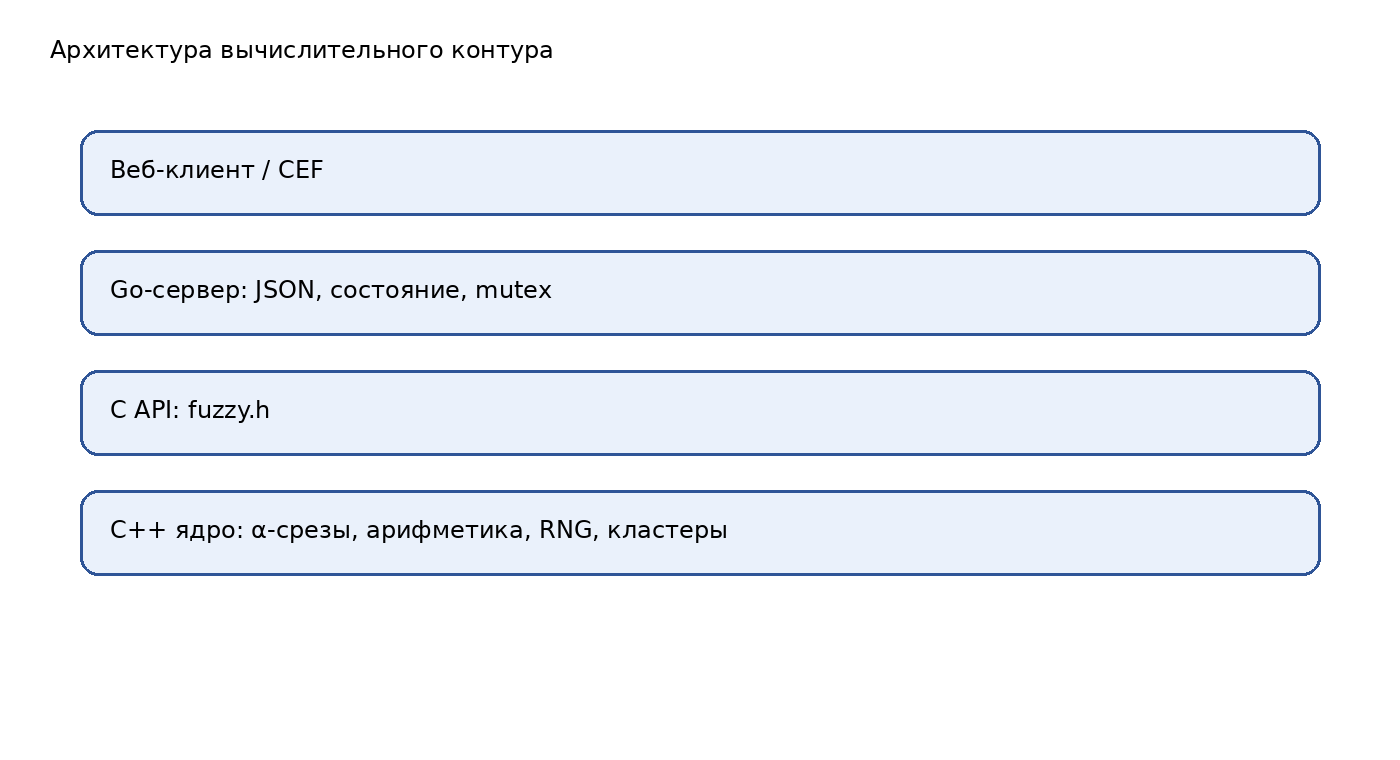
\includegraphics[width=0.9\textwidth]{figures/fig3_arch.png}\caption{схема архитектуры модуля кластеризации}\label{fig:3}\end{figure}

Сборка ядра описана в \texttt{fuzzy/CMakeLists.txt}. Создаются статическая \texttt{libfuzzy.a} и разделяемая \texttt{libfuzzy.so} из шести исходных файлов. Устанавливается C++17, включается position-independent code, применяются предупреждения \texttt{-Wall -Wextra}. Тестовый исполняемый файл связывается со статической библиотекой и регистрируется в CTest.

\subsection{Структуры данных C++}

\texttt{fz\_number} содержит флаг \texttt{uniform}, параметры \texttt{a} и \texttt{b}, а также векторы \texttt{left} и \texttt{right}. Для исходных U(a,b) параметры служат компактным каноническим представлением, а массивы хранят предвычисленные срезы. Для результатов операций \texttt{uniform=false}, параметры a и b не используются, а векторы описывают полную величину.

\texttt{fz\_set} содержит число уровней и \texttt{std::vector<fz\_number> items}. Вектор владеет объектами, поэтому освобождение набора освобождает все элементы без отдельного цикла в клиентском коде. Функция \texttt{fz\_set\_item} возвращает указатель, принадлежащий набору, и API явно запрещает освобождать его отдельно.

\texttt{fz\_rng} содержит четыре 64-битных слова состояния. Использование фиксированного размера исключает динамические аллокации в самом шаге генератора.

\subsection{Управление памятью и ошибки}

Объекты, созданные \texttt{fz\_create}, \texttt{fz\_create\_from\_cuts}, \texttt{fz\_clone}, операциями и генератором наборов, освобождаются парными функциями \texttt{fz\_free} и \texttt{fz\_set\_free}. Внутри ядра используются RAII-контейнеры \texttt{std::vector}, а C API предоставляет непрозрачные указатели. Такой контракт отделяет управление памятью C++ от Go-объектов.

Все функции, которые могут вернуть ошибку, очищают thread-local сообщение через \texttt{clear\_error}, затем записывают причину в \texttt{set\_error}. Go-функция \texttt{lastError} преобразует \texttt{fz\_last\_error()} в объект \texttt{error}. В HTTP-слое ошибки переводятся в JSON с кодом 400. В частности, отклоняются неверные диапазоны генерации, запросы с \texttt{a>=b}, неизвестные критерии, неверные методы и деление через ноль в носителе.

Журналирование синхронизировано мьютексом \texttt{g\_log\_mutex}. Каждая запись содержит локальное время, текст операции и немедленно сбрасывается в файл. Журналируются создание величин, арифметика, сравнения, генерация, отбор, кластеризация и ошибки.

\subsection{Реализация Go-оболочки и HTTP API}

В \texttt{server/fuzzy.go} через cgo подключается \texttt{fuzzy.h}, а параметры линейных массивов передаются в C как указатели на непрерывные участки Go-срезов. Функция \texttt{Generate} получает набор из C++ и копирует его в \texttt{[]Uniform}. \texttt{Intervals} создаёт временный C-набор, вычисляет срезы и копирует границы в два Go-среза. После возврата из функции C-объект освобождается через \texttt{defer}.

Сервер хранит \texttt{items}, \texttt{alpha}, массивы \texttt{left} и \texttt{right}, флаги отбора, метки кластеров, метод, число итераций и статистику кластеров. Все обработчики, изменяющие состояние, проходят через \texttt{handle}, который захватывает \texttt{sync.Mutex}, вызывает бизнес-операцию и формирует снимок \texttt{Snapshot}.

Основные маршруты имеют следующий смысл:

\begin{itemize}
\item \texttt{/api/generate} создаёт новый набор по seed и диапазонам;
\end{itemize}

\begin{itemize}
\item \texttt{/api/add}, \texttt{/api/clear}, \texttt{/api/import} изменяют набор;
\end{itemize}

\begin{itemize}
\item \texttt{/api/alpha} пересчитывает α-срезы без повторной генерации;
\end{itemize}

\begin{itemize}
\item \texttt{/api/select} применяет критерий ширины, окна или снимает отбор;
\end{itemize}

\begin{itemize}
\item \texttt{/api/cluster} запускает k-means++ либо пороговый алгоритм над выбранными интервалами;
\end{itemize}

\begin{itemize}
\item \texttt{/api/op} выполняет арифметику и сравнение двух U(a,b);
\end{itemize}

\begin{itemize}
\item \texttt{/api/export} выдаёт CSV с параметрами, срезами и метками;
\end{itemize}

\begin{itemize}
\item \texttt{/api/log} возвращает хвост журнала размером не более 256 KiB.
\end{itemize}

При любом изменении набора или α вызывается \texttt{recompute}. Он получает текущие интервалы из C API, выставляет все элементы выбранными и сбрасывает старые кластеры. Тем самым предотвращается использование меток, рассчитанных на другой α или другой состав данных.

\subsection{Веб-интерфейс и десктопный запускатель}

JavaScript-клиент строит графики на Canvas. Функции рисуют функции принадлежности, α-срезы, упорядоченные интервалы, плоскость (A,B), центры кластеров и результат арифметических операций. Данные поступают через JSON API и обновляют таблицы без перезагрузки страницы.

Десктопная часть использует CEF. \texttt{ServerProcess::Start} выбирает свободный loopback-порт, запускает \texttt{fuzzy-server} через \texttt{fork} и \texttt{execl}, ожидает доступность TCP-порта не более десяти секунд. Для корректного завершения дочернего процесса устанавливается \texttt{PR\_SET\_PDEATHSIG}, а при закрытии окна вызывается \texttt{Stop}, который сначала посылает SIGTERM и при необходимости SIGKILL. \texttt{FuzzyClient} обрабатывает заголовок окна, ошибки загрузки и загрузку CSV в каталог Downloads.

Такое разделение сохраняет единый вычислительный и серверный контур для браузерного и десктопного режимов. Различается только способ отображения страницы и жизненный цикл локального сервера.

\begin{figure}[htbp]\centering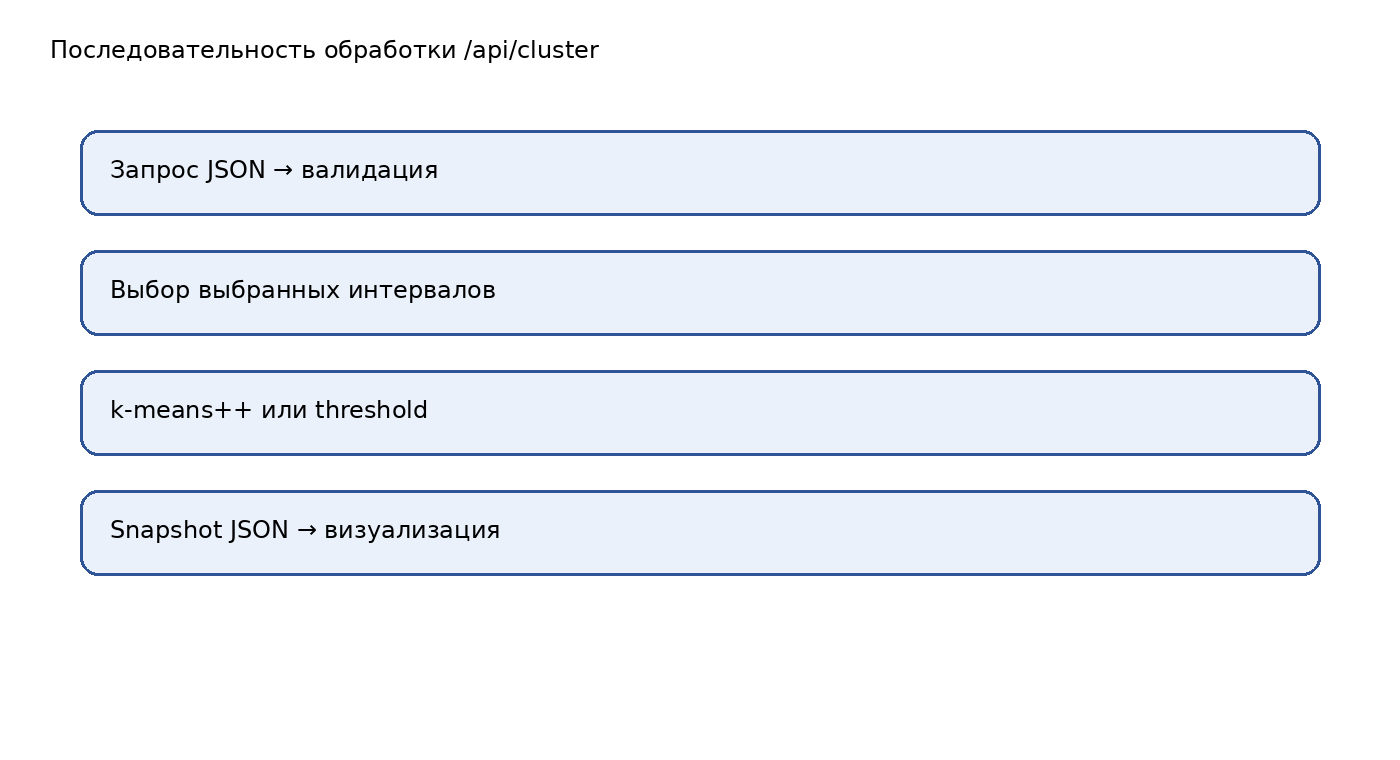
\includegraphics[width=0.9\textwidth]{figures/fig4_sequence.png}\caption{последовательность обработки запроса /api/cluster}\label{fig:4}\end{figure}

\subsection{Оценка вычислительной сложности}

Пусть n — число интервалов, k — число кластеров, m — число α-уровней.

\begin{itemize}
\item построение U(a,b) и вычисление одного α-среза имеют сложность O(m) и O(1) соответственно;
\end{itemize}

\begin{itemize}
\item получение всех α-срезов набора имеет сложность O(n);
\end{itemize}

\begin{itemize}
\item отбор по ширине и окну имеет сложность O(n);
\end{itemize}

\begin{itemize}
\item одна итерация k-means имеет сложность O(nk), а инициализация k-means++ — O(nk);
\end{itemize}

\begin{itemize}
\item пороговая кластеризация требует сортировки O(n log n) и до 50 проходов, каждый из которых в общем случае имеет сложность O(nk);
\end{itemize}

\begin{itemize}
\item расчёт статистики кластеров выполняется за O(n+k).
\end{itemize}

Память k-means составляет O(n+k), порогового алгоритма — O(n+k). Временная стоимость передачи через cgo определяется копированием результатов и не меняет асимптотику алгоритмов. Фиксированный размер 21 уровня в Go-сервере ограничивает объём JSON, тогда как C API поддерживает более плотную сетку.

---
